\documentclass[12pt,a4paper]{report}
\usepackage{graphics} 
\usepackage{graphicx}
\usepackage{amsmath}
\usepackage[english]{babel}
\usepackage{geometry}
\usepackage{hyperref}
\usepackage[utf8]{inputenc} 
\usepackage{listings}  
\usepackage{minted} 
\usepackage[table]{xcolor}
\usepackage{colortbl}
\usepackage{hyperref}  
\usepackage{enumitem} 
\usepackage{csquotes} 
\usepackage{longtable}
\usepackage[labelfont=bf]{caption} 
\usepackage{listings}
\usepackage{xcolor} 
\usepackage{multirow} 
\usepackage{multicol}
\definecolor{darkgreen}{RGB}{0, 128, 64}
\definecolor{dark}{RGB}{35, 35, 35}
\definecolor{orange}{RGB}{255, 69, 0}
\setlength{\parindent}{10pt}
\lstdefinestyle{mystyle}{
	language=Python,
	basicstyle=\ttfamily,
	keywordstyle=\color{blue},
	commentstyle=\color{darkgreen},
	stringstyle=\color{dark},
	numbers=left,
	frame=single,
	moredelim=**[is][\color{orange}]{@}{@},
}
\renewcommand{\lstlistingname}{Code Example} 
\definecolor{myblack}{rgb}{0.1, 0.1, 0}
\lstdefinestyle{stylepython}{
	backgroundcolor=\color{blue!8},  % Background color (adjust to your desired color)
	basicstyle=\ttfamily,            % Font style
	language=Python,                % Language (e.g., Python)
	numbers=left,                   % Line numbers on the left
	numberstyle=\tiny\color{myblack},  % Line number style
	breaklines=true,                % Automatically wrap long lines
	frame=single,                   % Add a frame around the code
	showstringspaces=false,         % Don't show spaces in strings
	keywordstyle=\color{myblack},      % Keyword color
	commentstyle=\color{myblack},     % Comment color
	stringstyle=\color{myblack}         % String color
}


%\renewcommand{\thepart}{\roman{part}}
\usemintedstyle{default}
% Define a style for Python code
\lstset{
	language=Python,
	basicstyle=\ttfamily\small, % Font size and style
	keywordstyle=\color{blue}, % Keywords font color
	stringstyle=\color{orange}, % Strings font color
	commentstyle=\color{gray}, % Comments font color
	showstringspaces=false, % Don't show spaces in strings
	breaklines=true, % Wrap long lines
	numbers=left, % Show line numbers
	numberstyle=\tiny\color{gray}, % Line numbers font style
	frame=single, % Add a frame around the code
} 

\geometry{left=2.5cm, right=2.5cm, top=2.5cm, bottom=2.5cm}
\begin{document} 
	\begin{titlepage}
	\begin{center}
		\LARGE{{\textbf{CATHOLIC UNIVERSITY OF BUKAVU}}}\\
		\begin{center}
			\begin{figure}[h]
				\centering
					\includegraphics[width=4cm, height=4cm]{"../../../../Latex Projects/ucb"}
			\end{figure}
			\large{\underline{B.P.285 BUKAVU}}
				\vspace{0.3cm}
		\end{center}
		\hspace*{0.5cm}
		{\large {\huge {\LARGE 	FACULTY OF SCIENCES  \textsf{}}}}\\ 
			{\Large \hspace*{0.7cm} Department of Computer Science}
			\vspace*{0.1cm}
			\setlength{\fboxsep}{4mm}
			\setlength{\fboxrule}{1mm}
			\vspace{0.5 cm}
			\rule{1\textwidth}{3pt}\\
			\vspace{0.18 cm}
			\begin{minipage}[c]{15cm}
				\begin{center}
					\LARGE{\textbf{\textcolor{black}{Development of a messaging application for communication and detection of spam on a mobile operator, case study of Airtel, Vodacom and Orange.}}}
				\end{center}
		\end{minipage}
	\end{center}
	\hspace{3pt}\rule{1\textwidth}{3pt}
	\vspace{0.1cm}
	\begin {minipage}{0.5 \textwidth }	
	\begin{flushright}
		{\large 
			\vspace {0.1cm} 
			\begin{tabbing}					
				\hspace*{1cm} \\
				\\
				\hspace*{2cm} Presented by : \textbf{MURHULA BYABUSHI Christian}  \\
				\hspace{2cm} \textit{Dissertation presented and defended in order to obtain the} \\
				\hspace{2cm} \textit{degree of Bachelor in Computer Science.}\\
				\vspace*{0.3cm}\\
				\hspace*{2cm} Option: Network and Telecommunications\\					
				\hspace*{2cm} Degree: Final year of Bachelor\\ 
				\vspace*{2cm}\\
				\\
				\hspace*{2cm}Supervised by: \textbf{\textit{Hw}. MUGISHO MUSHEGERHA Youen }\\
				\hspace*{2cm}Directed by : \textbf{\textit{PhD}. Elie ZIHINDULA}			
			\end{tabbing}
		}					

	\end{flushright}
\end{minipage}
\begin{center}
\end{center}

\begin{center} 
	\huge{\textbf{Academic year: 2022-2023}}
\end{center}
\end{titlepage} 
	\tableofcontents 
	\listoffigures
	\listoftables
	
	\newpage
	

	\addcontentsline{toc}{chapter}{Introduction} 
	\chapter*{Introduction}
	\section{Context and generalities} 
	With the increasing of use of mobile devices in mobile telecommunication, the number of text messages sent every day has grown exponentially. According to \textit{Statista}, a company that provides market and consumer data on a wide range of topics, including digital media and technology; the number of mobile messages sent worldwide in 2020 reached 3.5 trillion \cite{Statista2020}. 
	In the same case, with the raise of web pages and social media messaging applications like Whatshap, Teelgra, Snapchat Facebook, Instagram and many others, phone users can now send messages  that are only based on text as in former time but also on video, audios which are more chestful comparatively \cite{faklaris2016oh}. \\
	
	For sure, for interacting with his partner more professionally, email message is the most mean used, but not in all cases since in some countries a given SIM Card of a telecommunication provider is used as a bank more than being an communication mean, so the importance to secure the communication lines of a mobile users in these countries.
	Along with the functions and interests that the mobiles messages encompasses in terms of conversing, money sending and receiving, there has been an increase in the number of spam messages that aim to deceive people into providing personal information, sending unwillingly money, menacing to death or taking other actions that benefit the scammer.\\
		
	To address this problem, the development of a messaging application with advanced spam detection capabilities is crucial to set, filter messages and prevent the users. This dissertation focuses specifically on the development of such application for phone users and in general for mobile networks telecommunications technologies.  
	
	%such as : Airtel, Vodacom and Orange. \\
	% Indeed, Airtel, Vodacom, and Orange are major telecommunications operators which mostly function in Democratic Republic of Congo, with a significant market share and importance in online services, including messaging. 
	 
	\section{Problematic} 
	In telecommunication domain, we use mobile devices or phones for sharing \textit{SMS}, Email, chats by using some specific apps. Among all we use specifically \textit{SMS} for personal and professional information sharing \cite{lavanya2582sms}. The SMS stands for Short Message Service, which is a text messaging service for mobile phones and other mobile devices. It allows users to send and receive short messages of up to 160 characters \cite{le2005mobile}. It is also possible to send or receive automatic SMS which are not sent by human, whereas by using web interface or API \cite{jangir2016design}.
	
	Time to time, more persons are receiving messages such as : "You won x amount of money send another amount to withdraw it", "Join me at x area to take your money but pay me the transport ...", "I'm \textit{Sirene} Madam I have money for you", "I have a job for you" and many others fake messages. More of them are reported in this  \href{ https://blog.textedly.com/spam-text-message-examples}{spams examples link}.  
	
	Furthermore, scammers go the point where they can introduce vulnerabilities in messages which exploit a weakness in the SMS messaging system to remotely install spyware on mobile devices commonly called \textit{Simjacker}  \cite{cimpanu2019simjacker}. However, in marketing  almost similar messages are used to sensitize people to by products and services which confuse users wether it is or not a spam message by leading users to ignore important messages or being more hesitant to engage with mobile marketing campaigns \cite{chen2017survey},\cite{leppaniemi2008mobile}.
	
	Considering all above issues caused by spam, what are key technical challenges that could be addressed in messaging system which can effectively facilitate the communication as well as detecting and filtering spam messages ? 
	
	\section{Hypotheses}  
	 According to the Oxford dictionary, hypotheses stands for a statement of the expected relationship between things being studied, which is intended to explain certain facts or observations \cite{park2012dictionary}. An idea to be tested.
	 Hence, using the content-based filtering techniques, which involves analyzing the content of messages and determining wether it is a spam or not would be considered as solution. 
	
	 Firstly this would be done by utilizing the Machine learning algorithms which are : \textbf{Naive Bayes, Logistic Regression, and Supper vector Machines}. All these would be combined by the ensemble methods for making a more predictive model \cite{raschka2017python} including the preparation and classification techniques which avoid biased model \cite{karl1986model}. 
	 
	 Secondly, during the production steps, we should integrate the model inside of the system able to add technically in a blacklist or whitelist suspect users based on the specific probability of being a potential attack.
	 
	 Overall, we will jump from Machine Learning as model (\textit{MLaaM}) which is the output of writing ML algorithms run on data and represent what was learned by the algorithm on training data; to ML Model Software Deployment which encompasses all the activities that make a software system worthy to be used \cite{hadullo2021machine}.
	 
	\section{Delimitation and objectives}  
	\subsection{Delimitation}
	The present work aims to develop a messaging application for communication and detection of spam on a mobile network.
	
	Geographically it focuses on all provinces of Democratic Republic Of Congo(DRC) where mobile phones are used and require techniques for implementation. 
	
	Besides, it does not function effectively across all languages unless the solution model has been specifically trained on those languages. As a result, it is challenging to claim its effectiveness in languages such as Swahili, Lingala, French, or even English. Moreover, achieving optimal performance often necessitates the involvement of a large population.
	
	Indeed, the current work in terms of planning and execution has spanned a duration of nine months : From January to November 2023. 
	\subsection{Objectives}
	This system present 2 types of objectives such as: functional and non functional.
	
	As functional objectives, this system consist of developing a messaging application that can facilitate efficient communication between users; implementing the machine learning models which has the capacity of classifying the messages and preventing spam messages under a certain probability; designing and integrating a user-friendly interface for messaging application;  
		
	For non-functional objectives, it allows the user whose messaging application complies with relevant privacy laws and regulation to protect data information, reducing the attacks and frauds; Increasing the trustfulness of users and mobile services compagnie provider, optimizing the power resources of the user against threats posed by scammers. 
	
	\section{Interest} 
	Personally, this paper has allowed the author to gain knowledge and more experience in the field of mobile networks and messaging applications. 

	Socially, the developed system contributes to facilitating communication and reducing the impact  of spam messages, which can be annoying and stressful for citizens.
	
	Economically, this system of detection helps to save business server time and resources by filtering out spam messages allowing for more targeted marketing efforts. 
	
	Scientifically, the research achieved contributes to the advancement of the science in the domain of Mobile Networks, SMS messaging, and Machine Learning data processing and classification.
	
	\section{Research Methodology}
	Throughout this paper, the research methodology will be used to guide the study towards achieving its objectives. The research will adopt a descriptive research design to describe the development of a messaging application for communication and detection of spam on a mobile network. The study will focus on both qualitative and quantitative research methods \cite{creswell2014research}. The qualitative method will involve a literature review, interviews and analysis of collected messages. while quantitative method will focus on the development and testing of the messaging application.
	
	The research will be conducted in two phases. The first phase will involve data collection through a survey questionnaire that can be completed on website, or can be directly provided to the web interface (API) by the mobile phone users for collecting their experience with messages and especially spams. Thus, the data collected will be analyzed using descriptive statistics \cite{bluman2017elementary} to identify the common types of spam messages and the frequency of occurrence, languages inside, and other attributes.  
	
	The second phase will involve the development of the messaging application using the data collected from the survey and the analysis of existing messaging applications. The development of the application will be guided by the principles of agile software development by using Python (Django framework) for \textit{Back-end} and HTML,CSS and JavaScript for \textit{front-end}. Then,the application will  integrate the use of machine learning models based on selection's research of each other.
	
	The evaluation of the messaging application interface will be conducted using both quantitative and qualitative methods. The qualitative evaluation will involve the measurement of the application's accuracy and efficiency in detecting and filtering spam messages, on the other hand the qualitative evaluation will involve a user study to determine the usability and user experience of the application.
	
	\section{Work Plan (or Work Subdivision)}
	The work plan of this dissertation is divided into four parts. The first is the introduction, which provides a background information on the research problem.
	The second part consist of a situation analysis and assessment while the third part focuses on literature review and explanations on the methodology. Then the fourth part presents the practical result of this work. Finally the conclusion part summarizes the key findings and contributions of the study and presents limitations and provide recommendations for future research. 
		
	\chapter{Situation analysis and assessment on mobile phones}
	\section{Introduction}
	In this chapter, we will focus on various aspects that enhance the comprehensiveness and practicality of this dissertation. It includes explanations of mobile messaging architecture, machine learning models, and spam messages in mobile world. Additionally, it provides an analysis of the architecture used by network operators, highlighting both positive and negative aspects of their approach to message handling.
	\section{Presentation of the working framework and definition of key concepts}
	\subsection{Definition of key concepts}
	\begin{enumerate}[label=\alph*)]
		\item SMS(Short Message Service) :\\
		The Short Message Service is a basic service allowing the exchange of short text messages between subscribers \cite{mobilemessaging}. For supporting virtually all mobile devices, SMS is considered as a universal means of communication that enables users to communicate and function even though all users are not active simultaneously (asynchronous communication).
		\item Enhanced Messaging Service (EMS) : \\
		EMS has been created to allow the transmission of richer and more advanced messages. Unlike traditional SMS, EMS accepts not only text messages but also audios, melodies, and animations \cite{le2005mobile}.
	    
	    \item MMS (Multimedia Messaging Service):\\
	    MSS has been developed to facilitate the transmission of rich multimedia content in mobile messaging. Unlike SMS and EMS, MMS enables users to send not only text messages but also various types of multimedia files such as images, videos, audio recordings and even slideshows \cite{le2005mobile}.
	    \newpage
		\item Spam message: \\
		A spam message is understood as an unsolicited or undesired messages received on mobile phones which constitutes veritable nuisance to the mobile subscribers \cite{shafi2017review}. Clearly, this message can be sent with the intention of gaining financial benefits, collecting personal or organizational information such as security numbers, credit card details, or login credentials, and soliciting money by making false promises of future benefits or rewards that do not materialize. 
		
		\item Networks operators:
		The  networks operators refers to companies or organizations that provide and manage telecommunication networks. These operators own and operate the infrastructure, such as mobile networks, fixed-line networks, or internet service provider (ISP) networks, that enable the transmission of user's information to another user of the network \cite{ghezzi2015strategy} 
		
		\item Artificial Intelligence (AI) :
		 AI refers to the field of computer science that focuses on creating intelligent machines or systems that can perform tasks that would typically require human intelligence. For being practical, it encompasses algorithms, models and technologies that enable computers and machines to simulate human like cognitive processes such as learning, reasoning, problem-solving, perception and language understanding.  
		 
		 \item ML (Machine Learning)  : 
		 Machine learning is a subfield of Artificial Intelligence that focus on the development of algorithms and models that enable computers to learn from data and make decisions or predictions without being explicitly programmed\cite{smola2010introduction}. Clearly, when the data is labeled during the training, we refer to it as supervised model. If contrast, when the data is unlabeled and the model must discover patterns and relationships itself, it is an unsupervised model. Additionally, whenever it performs both the labeling  and discovering patterns tasks, it refers to a semi-supervised model. Furthermore, there is the last type called reinforcement. This one, is used to teach a computer or an AI agent how to make series of decisions in an environment. Just like, we learn to play the game better by playing it over and over.   
		 
		 \item NLP (Natural Language Process):
		 NLP is a subfield of Machine Learning that studies the human language and combing techniques from statistics, linguistics, life-hoods for making sentiment analysis, text classification, machine translation, question answering and text generation in a way that it can be understood computationally \cite{cambria2014jumping}. 
		  \end{enumerate}
		\subsection{Presentation of the working framework}  
		In the eastern party of DRC (South Kivu- and North Kivu) the usage of mobile phones has become more common, transforming communication and connectivity in the region. 
	The DRC itself is a large country, covering over 2,345,000 square kilometers with the eastern provinces of North and South Kivu spanning approximately 59,483 and 65,070 square kilometers respectively \cite{giswatch2018}. According to recent statistics from \textit{GlobalEdge} \footnote{ \href{https://globaledge.msu.edu/}{GlobalEdge}  : Created in 1994 by the International Business Center and the Eli Broad College of Business at Michigan State University (IBC), globalEDGE™ is a knowledge web-portal that connects international business professionals worldwide to a wealth of information, insights, and learning resources on global business activities}, an American company, around 95 million people were living in the DRC in 2022 \cite{monusco2015}, of which approximately 46.9\% had active mobile phones based on \textit{GSM} \footnote{\href{https://www.gsma.com/aboutus/}{GSMA}  (Global System Communications Association) : An industry Organization which represents the interests of mobile network operators worldwide created in 1982 to ease cooperation between countries deploying \textit{GSM} (Global System fo Mobile) technology.} research. \\ 
		
		
		In this context, it is observed that more people in cities use mobile phones compared to those in villages, primarily due to limited accessibility. A research study conducted by \textit{Target Canibet} \footnote{\href{https://www.target-sarl.cd/fr/content/etude-sur-la-telephonie-mobile-en-rdc}{Target Canibet: Reseach \& Consulting Group working in DRC. \url{https://www.target-sarl.cd/fr/content/etude-sur-la-telephonie-mobile-en-rdc} }}in 2015 focused on mobile connections in DRC cities including Bukavu, Goma, Kinshasa, Lubumbashi, and Matadi, found that among 1,000 people surveyed in each city, 9 out of 10 individuals were subscribed to a network operator. However, it was noted that approximately half of them subscribed to two operators, while a quarter subscribed to four operators, and 18\% used the services of a single operator.  
		
		Furthermore, the recent statistics made by \textit{DataReportal} \footnote{DataReportal: A online Company designed to help people and organizations all over the world to find the data, insights, and trends they need to make better informed decisions produced by Simon Kemp, \url{https://datareportal.com/reports/digital-2023-global-overview-report}}  in DRC shows that the mobiles users continues to increase exponentially, merely because of new services provided by internet and Telecoms Operators, at the point that since 2021 to 2022, it is has been reported 3.6 million of new users between 2021 to 2022, a report that proves how much mobile phones is inevitable in this last decades.
			
	   \subsection{Network coverage and infrastructure}   
	    In fact, two telecoms services exist in DRC such as : Fixed services (26\%) and Mobile services (74\%). The first one known as landline or wired services, involve the use of physical infrastructure; the second one which is popular is the mobiles services refer to telecommunications services provided through mobile networks.
	    According to the Congolese Regulatory Agency (ARPTC), the DRC has four mobile operators - Vodacom RDC,
	    Airtel Congo, Orange DRC and Africell DRC. Vodacom is the leader in the voice segment, with 35.2\% of the market,
	    followed by Orange (30\%), Airtel (23.9\%) and Africell (10.9\%). In the mobile internet market, Vodacom has 37.44\%, Airtel
	    31.25\%, Orange 28.14\% and Africell 3.17\% \cite{stateInternet2019}. 
	     	 \\
	     	     	        
	   Additionally, since the 190s, when the DRC witnessed the first installation of operator systems such as Celtel(now Airtel) and Vodacom, followed by Orange and Africell, the telecomunications sector has shown significant market growth, reaching 1 Billion in 2022\$ and expanding at a rate of 21\% per year according to  \textit{GlobalData} \footnote{\href{https://www.globaldata.com/store/report/drc-telecom-operators-market-analysis/}{GlobalData: Expert Company of Analysis, innovatove Solutions}}. 
	   However, this growth necessitates the updating of the infrastructure, which includes various generations of technologies, namely the second generation, third, fourth, and fifth(under development).\\
	   	   
	   In fact, the second generation have been deployed in various territories to enable more efficient \textbf{voice calls, data networks services, and introduce SMS for text messaging}. The infrastructure required for 2G networks includes the following equipments: 1) BTS(Base Transceiver Station) : Transmit and receives signals between mobile devices. 2) MSC(Mobile Switch Controller) : serves as the switching entity that connects calls between mobile devices. 3) BSC (Base Station Controller) :  manages multiples BTSs and controlling radio resources, managing handovers between cells and optimizing network performance, 4) AuC (Authentication Center) responsible for managing subscriber authentication and encryption keys to ensure communication between mobile devices and the network, 5) Home Location Register (HLR) the database that stores subscriber information such as phone numbers, authentication details, and service profiles, 6) Visitor Location Register (VLR) : The VlR is a temporary database that stores information about roaming subscribers within a specific area 7) MS (Mobile Station), including all the technologies used by the  users's handset and has two parts :\textbf{ Firstly, the mobile equipment which contains the radio equipment, the user interface, the processing capability and memory requirements for call signaling, encryption, SMS and the id of the mobile phone(equipment IMEI number). Secondly the Subscriber Identity module (SIM Card),} used in encryption of codes needed to identify the subscriber, storing subscriber's information, locate the user \cite{realWorldNetworks} as (+243 for each congolese number). \\
	   Indeed, all the 2G technologies covers a large distance varying between 1880MHz - 2700 MHz.\\
	      
	   Besides, the third generation appears as revolution, \textbf{allowing multimedia messages, voice calls data, faster data speed}; however it requires a significant upgrade from the previous generation. Thus, the equipment involved in 3G technology includes : 1) BTS (Base station Transceiver) : Which plays the same role as for 2G; 2) Node B: Responsible for handling the radio interface and connecting mobile devices to the core network; 3) Radio Network Controller (RNC) : Controlling the Node B and managing the radio resources 4) Mobile Switching Center (MSC): The MSC is the central switching entity in the network that \textbf{connects calls between mobile devices}; 5) Serving GPRS Support Node (SGSN) : Responsible for managing packet-switched data services services and handling mobility for mobile internet access; 6) Gateway GPRS Support Node (GGSN): It serves as interface between the mobile network and external networks like internet; 7) The Home Location Register (HLR) and Authentication Center(AuC): plays the same role as in 2G; 8) Operations Support System (OSS) : It provides and functionalities for monitoring and managing the 3G network. 
	   Indeed, the 3G is appreciated for enabling higher- speed services and covers different frequency bands depending on countries, ranging between 850Mhz - 1700 Mhz \cite{mishra2007advanced}.\\
	   
	   Additionally, the fourth generation, commonly referred to as LTE(Long-Term Evolution) represents a significant advancement over previous generations in terms of infrastructure and services. This generation introduces higher data speeds, improved capacity, and better perfomance for mobile communication and data services. The upgrades in infrastructure include: 1) BTS and MSCs : These components remain unchanged from the previous generation 2) Evolved Packet Core (EPC)  The EPC is a critical component of the 4G core network architecture which provides the packet-switched backbone that handles data traffic and ensures efficient data delivery between mobile devices and the internet or other networks; 3)  Radio Access Network (RAN): The Ran is responsible for the radio interface between mobile devices and base stations; 4) LTE (Long-Term Evolution) :  is the primary air interface enabling the high data speeds, low latency; 5) Back-haul Network : It connects base stations to the core network and internet infrastructure; 6) Spectrum Allocation: Hands over the mobile operator access to specific radio frequency bands; 7) Network Management System: These systems monitor and manage the 4G network, ensuring its smooth operation, performance optimization, and troubleshooting.
	   However, it's spanning or coverage of 4G networks on frequency bands allowed in each country based on their preferences, ranging from 700MHz to 2600 Mhz. The higher frequency bands generally offer faster data speeds but may have a shorter range, while the lower frequency bands can provide broader coverage but with slightly lower data speeds \cite{mishra2007advanced}.
	\subsection{Mobile Phone Models}  
	Since the mobiles phones are essential tools for communication, there is a wide range of popular mobile widely used by citizens of the DRC. The popular models come from various brands and offer a range of features to cater to different user preferences and needs. Some of the popular mobile phone models in DRC include \textit{ Techno, Itel, Infinix, Samsung, Apple, Huwaei, Itel, HTC, Motorola}. As it can be seen on the figure \ref{fig:mobilevendor}, according  to the  recent statistics conducted by \textit{Statistica},
	Samsung was the market leader in terms of share from January 2018 to November 2020, but in 2022, Tecno has emerged as the market leader.
	\begin{figure}
		\centering 
		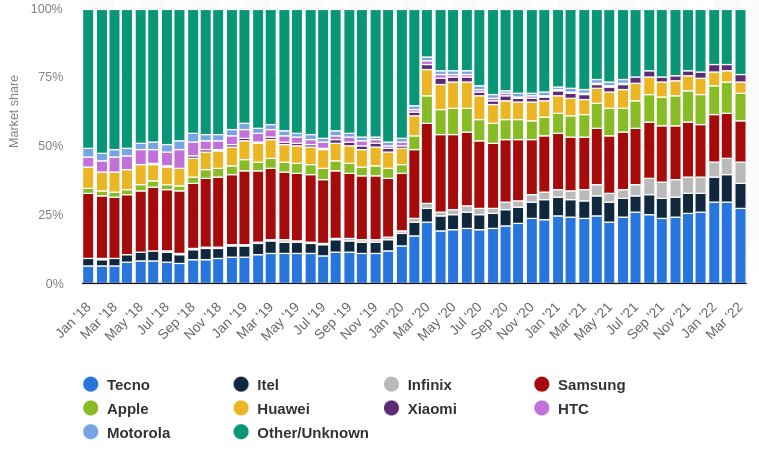
\includegraphics[width=1\linewidth]{Images/mobileMarket.png}
		\caption{Market share of mobile device vendors in the Democratic Republic of the Congo from January 2018 to March 2022}
	    \captionsetup{position=top}
		\label{fig:mobilevendor} 
	\end{figure}
\\

Furthermore, all these models provided above sell the telephone following different types which include mobile phones, offering the features such as touchscreen displays, cameras, internet, connectivity, and access to mobile apps; features phones, which are basic mobile phones used for calling and texting; smartphones used by the majority (around 35\% in DRC ), providing access to mobile internet, mobile apps, multimedia messaging, and various productivity tools; Tablets, used for reading and for the same functionalities as smartphones.
\subsection{Mobile usage and prevalence} 
In fact, each phone has its own unique set of characteristics that define its capacity and performance compared to others. Some phones come with specific applications that can be used independently, even without being connected to an operator, such as a camera, calculator, games app, and many others. However, other phones may not have such features.

To access the services provided by the operator, the phone's sim-card must be functioning, recognized by the operator, and capable of sending and receiving communication signals. \textbf{Of course, all these services work only if the phone's battery has sufficient power}.

Moreover, the services that citizen's subscribers benefit from are as follows : 

Firstly, the Internet Access: The Internet services are used to connect people from different nodes. In fact, In accordance with the \textit{WorldBank} \footnote{WorldBank : International Telecommunication Union ( ITU ) World Telecommunication/ICT Indicators Database \url{https://data.worldbank.org/indicator}}  been used by 23\% of the DRC's population in 2020. Nonetheless, it requires payment which proportionally gives mobile data usually expressed in Megabytes. 

Secondly, the Text Messaging (SMS): Even though the internet is the most used for texting, the SMS remains a widely used form of communication, especially in regions with \textbf{limited internet connectivity or among users who prefer simple text messaging or do not have the internet connection}.
Furthermore, with the architecture of GSM(Global System for Mobile Communications) invented in the second generation, sending messages became possible. Nowadays, the web environment has developed application interfaces (API) that connect external systems to operators for sending messages \cite{hassinen2003secure}. One of the platforms that offer these services connects its SMS gateway to the GSM operator, as seen in the case of \textit{Octopush} \footnote{Octopush : SMS platform for businesses connected with their audience} architecture shown in Figure \ref{fig:smsgateway}  

\begin{figure}
	\centering
	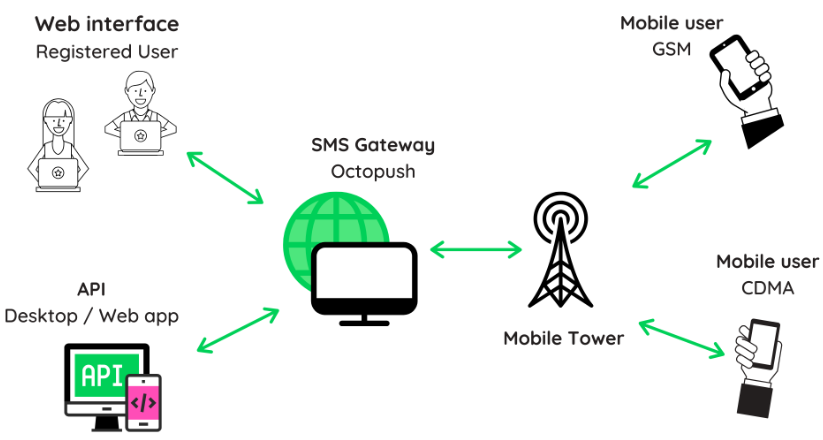
\includegraphics[width=1\linewidth]{Images/SMSgateway}
	\caption{SMS Gateway Provider Architecture}
	\label{fig:smsgateway} 
\end{figure}
    
Thirdly, the Mobile Banking and Payments : With this services subscriber can make \textbf{financial transactions}; paying bills, transferring money conveniently. 

Fourthly, the Mobile Entertainment: Mobile phones offer a range of entertainment options, from streaming videos and music to mobile gaming. 

And finally, the others Mobiles apps: This party includes the health services, education, social medias applications.
\section{Purposes of spammers in mobile messages}
Most of the time, spammers prefer to promise recipients prizes and then ask for money to claim the offer. They also attack SMS gateways with \textit{DoS} (Denial of Service) messages \cite{androulidakis2013fimess} whose goal is to overwhelm the system with unnecessary messages. Spammers send advertising and promotional messages based on company objectives, as well as SMS containing fake links or impersonating organizations to deceive recipients into taking certain actions or providing sensitive information \cite{tang2022clues}. Additionally, they may send SMS disguised as surveys to gather personal information for various fraudulent purposes.
\section{Solutions}
To address theses problems, it is necessary to involve various stakeholders, including network operators, app developers, regulatory bodies, and users. Firstly, it is recommended to implement mechanisms at the network level \cite{hao2009detecting} to filter messages and block users involved in spamming. Secondly, users (subscribers) should be educated on how to analyze messages and report any one that is causing disturbances. Thirdly, regulatory measures should be enforced to establish stringent regulations and penalties for spammers and those engaged in fraudulent mobile activities. Fourthly, the development of apps that enable filtering, classification, and reporting in the subscriber side would be beneficial. Fifthly, a website can be set to collect messages whether spam or ham reported by users who have doubts about their legitimacy, and then Machine Learning models can be used for detection purposes. For this, supervised or unsupervised methods can be employed to classify and predicting whether a message is spam or  ham. 
\section{Summary}
Overall, with the growth of mobile technologies, subscribers benefit from diversified services including : text messaging, voice calls, mobile baking, entertainment apps, and many others. However, These advancements also bring new challenges, such as the development of spam messages that aim to disturb network subscribers with unwanted or threatening messages. 

In DRC, especially in the eastern party, users face similar issues. This chapter emphasizes methods or techniques that can be used to address this problem and relatively reduce spam. One of the prominent techniques suggested is based on Artificial Intelligence, particularly Machine Learning algorithms.
    
    \chapter{Review of the Literature and description of the approach}
    \section{Introduction}
    This chapter delves into theory, methodologies, and machine learning techniques, including relevant algorithms and their deployment in the suggested solution. It also highlights the contributions of previous researchers in the field.  
    \section{Revue of the Literature}  
    Numerous researchers have extensively explored the subject of spam detection. Within this domain, some have directed their investigations towards the web environment, while others have delved into realm of mobile	technologies.
    
    Furthermore, these researchers have chosen to investigate the detection of spam across various communication channels, including emails and SMS, encompassing Multimedia SMS (MSS) as well. In the following sections, we comprehensively review the body of work that has been accomplished within this context as follows:
     
	\cite{katankar2010short}. \textbf{Dr.V.M Veena K.Katankar}
	proposed a system that comprises an SMS gateway for transferring SMS messages after they have been stored and encrypted by the web server. This software operates through a web interface. Whenever a client sends a \textit{POST} request, it is received by the web server, which is responsible for encryption or decryption if necessary. Subsequently, the gateway transfers the message as per its designated route. This solution proves to be particularly valuable in mobile banking and organizational marketing systems. Nevertheless, the author encourages other researchers to delve into channel services in communication and advanced encryption techniques.\\
		
	\cite{brown2007sms} In their publication titled \textbf{\textit{Short Message Service}}, \textbf{Brown, Jeff and Shipman} members of IEEE, delve into several significant aspects. They start by exploring th growth of mobile phones and SMS services. They also examine the system architecture of SMS Centers and technologies used for message communication
	
	Furthermore, they shine the spotlight on aggregators and services providers. These are the entities that enable users to send bulk messages, essentially sending messages with a large amount of text to a group of recipients. This includes the interesting capability of converting email messages into SMS.
	
	Moreover, the article highlights that some of these aggregators may choose to collaborate with cellular networks. In this collaborative role, they act as intermediaries, connecting third-party entities that don't have direct relationships with cellular service providers. To achieve this, they employ a \textit{SMPP (Simple Messaging Peer to Peer)} protocols.\\
	
	\cite{medani2011review} \textbf{Researchers A. Medani and A. Gani}, affiliated with the University of Malaysia, have published a comprehensive review focusing on security concerns and techniques related to mobile Short Message Service (SMS).
	
	In their paper, they illuminate the process by wich a subscriber sends a message to another party while adhering to specific principles of the Over-The-Air (OTA) structure. This process involves transmitting the message from the sender to the base station and then forwarding it to the intended recipient trough the SMS Center (SMSC).
	
	Crucially, they emphasize the importance of securing every SMS using \textit{Public Key Infrastructure (PKI)}, ensuring end-to-end transmission security and safeguarding the message from unauthorized modifications. However, it's worth noting that the use of PKI can potentially impact mobile device performance due to the significant power requirements for the encryption process, and it may not guarantee integrity across all standards.
	
	To address these security concerns within GSM systems, the researchers propose the implementation of \textit{XML Key Management Specification} as a middleware solution. This middle ware system servers an intermediary, facilitating secure communication between mobile devices and enhancing overall system security for the benefit of clients.\\
	
	
	\cite{crawford2015survey} \textbf{Nikhil Kumar}, a reseacher affiliated with the University of New Delphi in India, published an article focusing on the topic of Email Spam Detection Using Machine Learning. In his study, he placed particular emphasis on comparing various machine algorithms, including \textbf{\textit{Naive Bayes, Support Vector Classifier, AdaBoosting, K-Nearest Neighbour, and Bagging Classifier}}. The objective was to predict wether an email was categorized as spam or legitimate (ham). To demonstrate his approach, he utilized an existing dataset available in the Kaggle workspace.
	
	Through experimentation and parameter tuning, Nikhil found that Naive Bayes delivered promising results in terms of accuracy. However, he also pointed out a limitation associated with the Naive Bayes algorithm. This limitation is tied to its assumption of class-conditional independence, which implies that each feature is considered independent of the presence of the other features. In cases where this assumption does not hold, it can lead to misclassification of data points.
	
	To address this limitation and enhance the performance of spam detection, the author recommended the use of \textbf{ensemble methods}. These methods involve the use of multiple classifiers for making class predictions, allowing for more robust and accurate results.\\
		
	\cite{navaney2018sms} In 2018, researchers Pavas Navaney, Gaurav Dubey, and Ajax Rana, who are affiliated with the University of Southern California and Amity presented a conference paper titled "SMS Spam Filtering using Supervised Machine Learning Algorithms".
	
	Their study concentrated on a dataset comprising 5574 records, of which 4827 messages were categorized as "ham" (legimate messages), while 747 messages were classified as "spam" (unsollicited or unwanted messages).
	
	The researchers applied three different machine learning methods to this dataset. Among these methods, it was observed that the \textit{Support Vector Machine (SVM)} algorithm achieved the highest accuracy compared to the Naive Bayes and Maximum Entropy Classifier algorithms. \\
	
	\cite{shirani2013sms}  \textbf{Houshmand Shirani-Mehr}, a researcher in Machine Learning, published an article in 2013 titled : "SMS Spam Detection using Machine Learning Approach". His purpose was to address the spam filtering problem by utilizing ML algorithms. Therefore, He utilized a dataset from the  \textit{UCI Machine Learning Repository} repository \footnote{\textbf{UCI ML} : The UCI Machine Learning Repository is a popular collection of datasets maintained by the University of California, Irvine (UCI). It serves as a valuable resource for researchers and practitioners in the field of machine learning and data mining. \url{https://archive.ics.uci.edu/}} , which contained real SMS messages. In development, he employed the algorithms to tackle that problem such as :  Naive Bayes with Laplace smoothing, Support Vector Machine, and Ensemble methods (\textit{AdaBoosting and Random Forest}). As an improvement, the author added meaningful features such as the length of messages in terms of the number of characters and certain thresholds.
	
	The results obtained after applying these methods to the dataset indicate that the SVM algorithm achieved the highest accuracy score.
	\\
	
	\cite{gupta2021sms} The authors of the article titled "SMS Spam Detection Using Machine Learning", namely
	\textbf{Gupta, Suparna Das and Saha, Soumyabrata and Das, Suman Kumar}. Their focus was on reviewing various techniques employed by other researchers in the realm of machine algorithms for SMS spam detection. 
	
	In their research, they adopted a similar approach by incorporating the \textit{TF-IDF (Term Frenquency-Inverse Document Frequency)} method. This technique assesses the frequency of a word within a document and evaluates its importance in that document. \textit{TF-IDF} is a well-known method for measuring word relevance in a collection of texts.
	
	To assess the effectiveness of these techniques, the authors applied them to a spam dataset obtained from \textit{Kaggle} 
	\footnote{ \textbf{Kaggle :} a platform for data science competitions and datasets. \url{https://www.kaggle.com/}}
	. After conducting their experiments and evaluations, the authors arrived at a noteworthy conclusion. They found that among all the ML algorithms they employed, the Naive Bayes algorithm consistently achieved the highest level of accuracy in SMS spam detection.\\
	
	As shown above, many researchers have investigated the same topic using different approaches. Some have focused on security within mobile architecture, including message transfer processes, while others have concentrated on using Machine Learning (ML) models to combat the issue of spam. In general, these approaches are valuable to this project and serve as its inspiration at the point that many techniques related to these approaches have been implemented in this project.\\

    However, what sets this project apart is its pratical approach involving specific society. Rather than solely relying on existing datasets from platforms like \textit{Kaggle and UC Machine Learning Repository}, this project has actively engaged with people to collect data. It has also integrated some data from these platform datasets to enhance the quality of information. \\
        
    Furthermore, this project harnesses the latest advancements in machine learning. It utilizes Ensemble Methods to achieve high levels of accuracy. Addionnally, it employs technical parameter tuning, including \textit{GridSearcher and VotingClassifier}. In fact, GridSearcher assists in identifying the most suitable parameters required for algorithm models.  
    \\
    
    Moreover, this project doesn't stop at model development, it extends to the deployment of the models generated through the processes. It provides backend \textit{APIs} for certain platforms interested in learning from these results. 
    
    Additionally, it outlines the structure of GSM deployment, encompassing the SMSCenter's role in the mobile messaging system.
   
   
    
   \section{Tools and Techniques} 
	In the mission of this project to create a messaging application that not only streamlines mobile communication but also tackles the pervasive issue of spam, this section serves as a technical guide. It will explore the tools and techniques at the core of the approach used. \\
		
	Building an effective messaging application is like constructing a house- you need the right tools. Thus, this section discusses the software and technologies that form the foundation of our messaging app, including the programming languages, frameworks, and platforms utilized. \\
	
	To combat spam effectively, this project is enlisting the help of machine learning. It delves into the world of data analysis and machine learning tools and frameworks : \textit{numpy, pandas, matplotlib, scikit-learn,} that empower the authors to analyze, detect and prevent spam messages.\\
	
	\subsection{Messaging application development tools}
	In the realm of modern software development, the choices of development tools can significantly impact the efficiency and effectiveness of the project. When crafting application, the authors carefully considered the tools that will shape the foundation of the \textit{backend} and \textit{frontend} development. Actually, the \textit{backend} references the environment where data of the app are stored, structured and more secured; while the \textit{frontend} involves the space where techniques are developed to show to the user the interface comfortable for his understanding. Among all tools, some serve as programming languages and others as editors. 
	
	Hence, The choices made by the authors are \textit{Python (with Django \textit{Framework})} as programming language and \textit{SQL} for data structuring language in \textit{backend} development and HTML, CSS and Javascript (with \textit{Vue-Js Framework}) for \textit{frontend} environment. \\
	
	\subsubsection{Back-end Development with \textit{Python} (\textit{Django}) and \textit{SQL} :}  
	
\includegraphics[width=0.2\linewidth]{pythonImage.png}
	 is a powerful language appeared in 1980 firstly implemented by Guido van Rossum at \textit{Stichting Mathematisch Centrum} in the Netherlands as a successor of a language called  \textit{ABC} \cite{tulchak2016history}. It newest version is \textit{Python 3} \footnote{Python : \url{https://www.python.org/}}  which is available for all most environments, either \textit{Macos} or \textit{Linux} and \textit{Windows}.
	 
	 In comparison with \textit{Java, C, C++, MATLAB}, \textit{Python} is more readable, since it requires few lines of code which are clean. Next, it is a good choice for those who want to start with programming \cite{bogdanchikov2013python}. Technically it is versatile, since it used for a wide range of applications, from web development to mobile apps (with Kivy \footnote{Kivy: \url{ https://realpython.com/mobile-app-kivy-python/}} ), data analysis, machine learning, and scientific computing. Actually, the high reason that influenced the use of this programming language is its capacity to deal with data by proving scientists with many libraries. \\
	 
	 Since the frameworks help to gain time in terms of development and structuring a project, \textit{Python} provides many frameworks for web development. Notable these are Django, Flask, and more. Authors's choice, Django, is a high-level, open-source web framework for building robust and dynamic web applications. It's written in \textit{Python}, which is one of the reasons for its popularity. It follows the \textbf{\textit{batteries-included}} philosophy, providing a wealth of built-in features like authentification, URL routing, a powerful admin interface, and an ORM (Object-Relational Mapping) system, which simplifies database operations \cite{alchin2013pro}. \\
	 
	Actually, Django's ORM abstracts many \textit{SQL} complexities, enabling developers to interact with the database using \textit{Python} code, without needing to write raw \textit{SQL} queries. This higher-level interaction simplifies database access and makes the development process more efficient. So, while \textit{SQL} is at core of database interaction, Django's \textit{ORM} providers a user-interface for developers, streamlining the development of data-driven web applications.\\ 
	Suppose we want to retrieve all the employees in a database with salaries greater than \$4000 using raw SQL. Here's what the SQL query would look like : 	
\begin{lstlisting}[style=stylepython]
 SELECT * FROM employees WHERE salary > 4000
\end{lstlisting}
  While Django accomplishes the same task using the following code:
\begin{lstlisting}[style=stylepython]
from myapp.models import Employee
  employees = Employee.objects.filters(salary__gt = 4000)
\end{lstlisting}
    \subsubsection*{How did we get there ?}
   In fact, the project must be running for doing that. For installing \textit{Python}, just go to the official website for the  download, no matter the OS version, either \textit{ \href{https://www.python.org/downloads/macos/}{MACOS} , \href{https://www.python.org/downloads/windows/}{Windows} } or \href{https://www.python.org/downloads/source/}{\textit{Linux/UNIX}} since \textit{Python} is portable. Indeed, the last version at the writing of this project was Python 3.12.0. To test if the it is working, just enter the command \textcolor{blue}{python} as in figure \ref{fig:testpython}.
   \begin{figure}
   	\centering
   	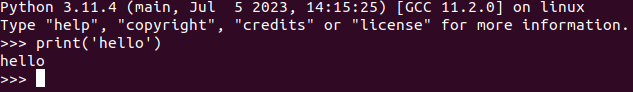
\includegraphics[width=1\linewidth]{testPython}
   	\caption{Testing if python is running on the OS (LINUX)}
   	\label{fig:testpython}
   \end{figure}
   
   
   Next, for installing Django, the steps remain pretty the same, going on the official page and following the guides as resumed in the as follows:   
   For the step 1, Installing the virtual environment ( \textit{V.M}) \footnote{How to create the VM ?https://realpython.com/python-virtual-environments-a-primer/}    : \newline
   \textbf{In Windows} : \texttt{python -m venv myenv}; then active it by : \texttt{myenv\textbackslash Scripts\textbackslash activate} \newline
   The word \textit{myenv} is just the name of virtual environment. But Why do we create it ? In fact, it is a best practice in Python development to manage dependencies, isolate projects, and maintain a clean and organized development environment. \newline 
  In \textbf{MACOS/Linux} : Only the way of activating the \textit{VM} changes. Then just by entering the following command:\newline
  \texttt{source myenv/bin/activate}; the virtual will be functioning. 
  \newline
   \textbf{Finally}, as the \textit{VM} is working Django, can be installed, by the command :  \texttt{pip install Django}. At the writing of this project, the last version 4.2.6. The bit steps to follow for installing are demonstrated in the figure \ref{fig:installdjango}
\begin{figure}
	\centering
	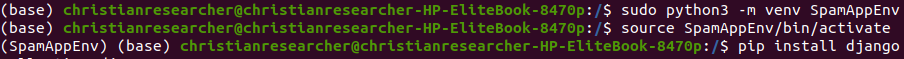
\includegraphics[width=1\linewidth]{installDjango}
	\caption{How to install django ? Here, the name of \textit{VE} is SpamAppEnv}
	\label{fig:installdjango}
\end{figure}
\\
 Now, the project can be created, followed by the app inside, depending on interests. For that the commands  : \textcolor{blue}{ \texttt{django-admin startproject projectname}} and : \textcolor{blue}{\texttt{django-admin startproject appname}} can be utilized. The result is demonstrated in figure \ref{fig:visualstudio}. 
\begin{figure}
	\centering
	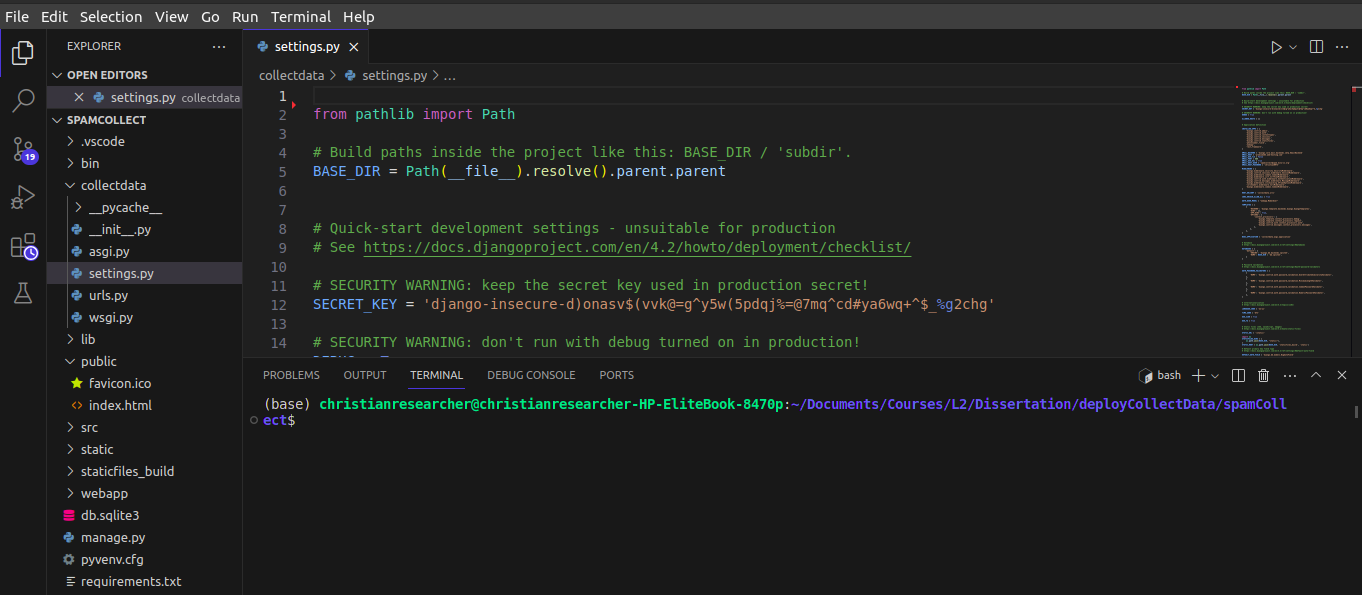
\includegraphics[width=1\linewidth]{visualStudio}
	\caption{After the project and app are already created}
	\label{fig:visualstudio}
\end{figure} 
 \newline However, the configuration about the app created, ought to be made lest it should raise the error. Thus, in settings file, present in the project folder the properties called \textit{INSTALLED\_APPS}, as in the figure \ref{fig:appinstallname}.\newline After, this we can just enter the commands : 
 \begin{lstlisting}[style=stylepython]
 python manage.py makemigrations
 python manage.py migrate
\end{lstlisting}
For sure, the first command line says to Django the new changes, and the second applies or assesses them. 
\begin{figure}
	\centering
	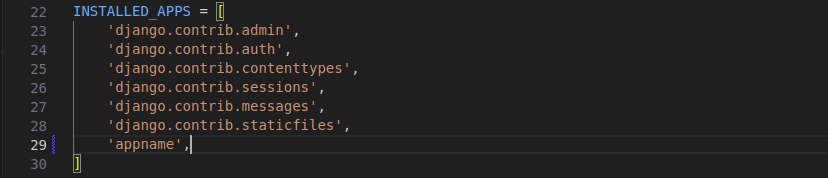
\includegraphics[width=1\linewidth, height=3.5cm]{appInstallName}
	\caption{Adding the appname in \textit{INSTALLED\_APPS} dependencies }
	\label{fig:appinstallname}
\end{figure} 

\subsubsection*{How does Django deal with the database ?} 
Django deals with databases through \textit{ORM} as mentioned above. Its management involves to follow different steps such as:

\textbf{Database Configuration } : in the Django project's settings (usually in the \textit{settings.py}, we have to specify the database we want to use. Django supports various databases types, including \textit{PostgreSQL, Mysql, SQLite and Oracle} \footnote{Setting Databases in Django : \url{https://docs.djangoproject.com/fr/4.2/ref/databases/\#mysql-notes}}  . We have only define the database backend, connection details, and other options in the \textit{DATABASES} setting. For instance the configuration of \textit{MYSQL} will be like this : 
\begin{lstlisting}[style=stylepython]
DATABASES = {
  'default': {
  'ENGINE': 'django.db.backends.mysql',
  'NAME': 'the_db_name',
  'USER': 'the_db_user',
  'PASSWORD': 'the_db_password',
  'HOST': 'localhost',  # or the IP address of the MySQL server
  'PORT': '3306',  # MySQL default port
 }
}
\end{lstlisting} 

\textbf{Model Definitions} : \textit{Django} models are Python classes that define the structure of the database. Models are defined in the the \textbf{\textit{models.py}} file. Each model class represents a database table, and each model field represents a table column. The syntax used for creating a database is as follows: 
\begin{lstlisting}[style=stylepython]
from django.db import models
class Employee(models.Model):
     name = models.CharField(max_length=100)
	     salary = models.DecimalField(max_digits=10, decimal_places=2)
\end{lstlisting} 
The corresponding \textit{SQL} code is this:  
\begin{lstlisting}[style=stylepython]
	CREATE TABLE Employee (
	 id INTEGER PRIMARY KEY,
	 name VARCHAR(100),
	 salary NUMERIC(10, 2)
	);
\end{lstlisting}  

 \textbf{Migrations} : Every time a model (database table) is created or modified, \textit{Django} need to notified for assessing these changes. As mentioned earlier, the command'\textbf{python manage.py makemigrations}' is executed in the terminal for managing the changes,  '\textbf{manage.py migrate}' command is entered to apply all of these changes.   \\
 
\textbf{Database abstraction} : With this technique, we do'nt no longer need to write \textit{SQL} code, since by \textit{Python} it is possible to interact with the database, and making a \textit{queryset} request(\textit{crud}  \footnote{CRUD: Create Read Update Delete item}).Let's see how it works once again: 

\begin{lstlisting}[style=stylepython]
new_employee = Employee(name ="Eistein", salary=45OOOO) 
new_employee.save()
\end{lstlisting} 
instead of doing this in SQL : 
\begin{lstlisting}[style=stylepython]
INSERT INTO employees (name, salary) VALUES ('Einstein', 45000);
\end{lstlisting}  

Indeed, we can see that even a non-professional in \textit{SQL} can now deal with the database without any \textit{SQL} code. \newline
Furhermore, the use of abstraction techniques to interact with database, enhances its security of by guarding against \textit{SQL injection}. 
\subsubsection{How does Django do for interacting with APIs ?}

\textit{Django} presents a useful package for interacting with the \textit{API} called \textit{DRF \footnote{DRF (Django Rest Framwork) : a powerful tools serving to interact with Apis. \url{https://www.django-rest-framework.org/}}} It allows : authentication policies including optional packages for \textit{OAuth1a} and \textit{OAuth2 \footnote{OAuth2 :   (Open Authorization 2.0) : is a framework that allows third-party applications to access a user's data without exposing their credentials, such as passwords.OAuth 1.Oa is the old version of OAuth2  }}, web browsable API  and serialization \footnote{Serialization : converting data into formats like \textit{JSON}, \textit{XML}, etc. The deserialization involves the reconstruction of the same operation} and deserialization that supports both \textit{ORM} And \textit{NO-ORM} data sources \cite{nader2023django}. 
 
\subsubsection{\large \textit{Front-end} Development with \textit{HTML}, \textit{CSS} and \textit{Js} :} 
The Front-end development is a crucial aspect of web development that focuses on creating the user interface and user experience of a website or web application. It involves using a combination of HTML,CSS, and Javascript to build the visible and interactive elements of a website. 

The HTML (Hypertext Markup Language) is used as a maker of web pages by providing its structure and content. It uses a markup language with various tags to define headings, paragraphs, links, images, forms, and more \cite{stark2010building}. For example a page with a heading and a paragraph should look like this in the content :
\begin{lstlisting}[style=stylepython]
 <div>
     <h1>Page Dev</h1>
     <p>this is our page</p>
 </div}
\end{lstlisting}

Furthermore, the \textit{CSS (Cascading Style Sheets)} is used for styling and layout. Thus, it controls the visual presentation of HTML elements. For example for our above code : \newline
\begin{lstlisting}[style=stylepython]
h1{
   color : blue; /* set the color to the element*/
   font-size: 24px; /* sets the font size */
   text-align: center; /* centers the element*/
}
\end{lstlisting} 

Apart from that, the other powerful tool used in web development is \textit{JS(JavaScript)}. It adds interactivity and dynamic behavior to web pages. It also leveraged for creating features like images sliders, form validation, animations and real-time updates without having to \textbf{reload the page}. The common frameworks used to extend its productivity are : React, Angular and Vue-js \cite{wohlgethan2018supportingweb}. By updating the above \textit{HTML} code, we can see the interactity created by JS: 
\begin{lstlisting}[style=stylepython, label=lst:jsCode]
<!DOCTYPE html>
<html>
<head>
 <title>JavaScript Example</title>
</head>
<body>
 <div>
 <h1 id="pageTitle">Page Dev</h1>
 <p>this is our page</p>
 </div>
	
 <button id="changeTitleButton"  onclick="changeTitle()">Change  Title</button>
	
 <script>
 	// JavaScript function to  change the title
 	function changeTitle() {
 	// Get the h1 element by its ID
 	var titleElement =  document.getElementById("pageTitle");
	
 	// Check if the element exists
 	if (titleElement) {
	// Change the text of the h1 element
 	titleElement.innerText = "New Page Title";
	  }
	}
 </script>
</body>
</html>	
\end{lstlisting} 

In this example, the button with the ID 'ChangeTitleButton' and the function called 'ChangeTitle()' are added. The click on the 'Change Title' button executes the changeTitle function. Then, the function retrieves the \texttt{<h1>} element by its
ID ("pageTitle") and changes its text to "New page Title". Thus, by this bit snippet code, \textit{JavaScript} really appears interactive.

\subsection{\large Machine Learning tools and frameworks} 
Machine learning involves learning from data, visualizing, analyzing it, and making predictions. To do this, we need the right tools. \textit{Python} is one of best and powerful tools used for these tasks. It has a large and active community that continuously contributes to its growth. \textit{Python} offers a variety of packages that assist data scientists in their work.

In Python, common packages used for working with data include\textbf{ numpy, pandas, matplotlib, seaborn, scikit-learn, tensorflow}, and more.

The Integrated Development Environment (\textit{IDE}) used for working in Python, even for all backend-development is : Visual studio. It is portable and downloadable from the official page( \url{https://code.visualstudio.com/}). Additionally, we have another \textit{IDE} called \textit{Anaconda} including \textit{Jupyter notebook} which is used for machine learning and data science projects. It's designed to simplify package management and deployment by using a package manager called \textit{Conda} which helps users to install, update, and manage packages, libraries and dependencies \cite{teimourzadeh2022application}.

To start a new project we just execute in the terminal, the command :  \texttt{jupyter notebook}, then a default browser configured just open directly the link. The page look like in the fig \ref{fig:jupyteropen}.
\begin{figure}
	\centering
	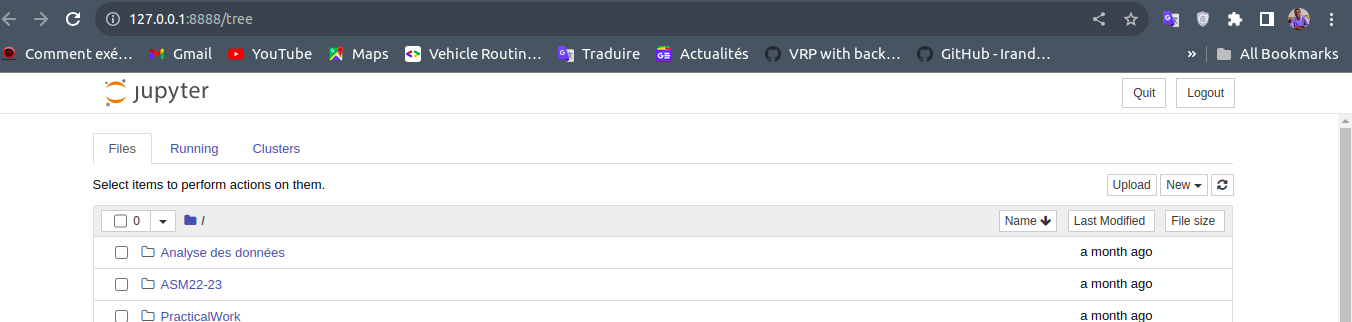
\includegraphics[width=1\linewidth]{jupyterOpen}
	\caption{Start jupyter in conda kernel}
	\label{fig:jupyteropen}
\end{figure}  

\subsubsection{{\large Data manipulation with \textit{Numpy}, \textit{Pandas}}}
  \textit{\textbf{Numpy}} Library
 
   \textit{Numpy} is a fundamental library for scientific computing with Python. It provides support for large, mutli-dimensional arrays and matrices, along with an assortment of high-level mathematical functions to operate on these arrays.\newline 
 Actually, the reason of thinking about a new tool of computing in Python is because, all  data structures it provides: lists for enumerating a collection of objects, dictionaries to build hast tables, are not ideally suited to high-performance numerical computation \cite{van2011numpy}.\newline 
 Basically, the usage of numpy asks for importing its modules like this :  
 \begin{lstlisting}[style=stylepython]
 import numpy as np  #np is a common alias used  
 In [4]: np.__version__
 Out [4] : '1.24.3'
 \end{lstlisting} 
 %% We assume that the np alias created will be used for other demonstration.\newline
 \textbf{The structure and creation of a \textit{NumPy} array}. The fundamental data structure provided by the Numpy library for representing arrays is \textbf{ndarray} it refers to the array which is n-dimensional or multi-dimensional \cite{coursAnalyseDonne2}. Thus, several means can be used to create an array as follows  : \newline
 - With 1D(dimension):
 \begin{lstlisting}[style=stylepython]
In[8] : np.array([1, 2, 3, 4, 5])
#Creates a NumPy array from a given list or iterable.
Out[8] : array([1, 2, 3, 4, 5]) 

#2D array
In[12] : np.array([[1, 2, 3], [4, 5, 6]])

In[12]: array([[1, 2, 3],
		[4, 5, 6]])
 \end{lstlisting}
 \begin{lstlisting}[style=stylepython]
In[10] : np.arange(1, 10, 2)  
# Creates a 1D array from 1 to 9 with a step of 2
Out[10] : array([1, 3, 5, 7, 9]) 
#2D array for arange function, requires manipulation
 \end{lstlisting} 
  Many other functions can be used for creating arrays, like : empty, zeros, ones, eye, etc. \\
  
 \noindent\textbf{Manipulation of arrays}. The manipulation operation includes : The splitting, slicing, indexing,reshaping, arithmetical operations, concatenations, comparisons and many others. Let's dive into some of that operations as follows:
 \begin{lstlisting}[style=stylepython] 
 #We generate the integers from zero to twelve and
 # re pack them into a 4x3 array
 In [21] : np.arange(12).reshape((4,3))  
 Out [21] : array([[ 0,  1,  2],
 		    [ 3,  4,  5],
 		    [ 6,  7,  8],
 		    [ 9, 10, 11]]) 
 #Suppose we want to multiply each vector element by 3
 In [24] :  a = [3,7,4] 
           [4*x for x in a]
 Out[25] : [12, 28, 16]  
 #Concatenate arrays vertically  
 In [29] : np.vstack(([1, 2, 3],[1, 2, 3]))  
 Out [29] : array([[1, 2, 3],
                   [1, 2, 3]]) 
 #Concatenate arrays horizontally
 In [31] : np.hstack(([1, 2, 3],[1, 2, 3]))
 Out [31] : array([1, 2, 3, 1, 2, 3])   
 
 
 \end{lstlisting} 
 Let's mention that ndarray object is homogeneous since all elements within must have the same data type. The types allowed are : Float, int, bytes, str, number and complex (for decimal complex numbers). To define, the type on the array on creation is made by \textbf{dtype} property like this: 
\begin{lstlisting}[style=stylepython] 
 In [55] : np.array([1, 2, 3, 4, 5], dtype='float') 
 Out [55] : array([1., 2., 3., 4., 5.]) 
\end{lstlisting} 

Besides, dealing with slicing and splitting still depends on the dimension. Lets break in the code to see that : 
\begin{lstlisting}[style=stylepython]
In [56] : arr = np.array([[1, 2, 3],
[4, 5, 6],
[7, 8, 9]]) 

#split along rows (axis=0)
In [59] : split_rows = np.vsplit(arr, 3) # Split into threee 1-row arrays
Out[59] : [array([[1, 2, 3]]), array([[4, 5, 6]]), array([[7, 8, 9]])]

#slicing 
In [60] : arr[1:3, 1:3]  # Get a 2x2 subarray
Out [60] : array([[5, 6],
		  [8, 9]])
\end{lstlisting}   
 Some others functions are used as follows : all, any, cov-corrcoef, dot, where, random(), randint() and many others. The details of usage are given on the official of Numpy package \footnote{Numpy, official page : https://numpy.org/}.
\\

\subsubsection*{{\large  Pandas library :}} 
\textit{Pandas \footnote{https://pandas.pydata.org/} } is an essential open-source Python library used for data manipulation and analysis. It provides functions for reading and writing data structures in various formats, including \textit{CSV} and text files, Microsoft Excel, SQL databases, and the fast \textit{HDF5} \footnote{HDFR (Hierchical Data Format version 5) : It is a versatile and high-performance data storage format commonly used in scientific and data analysis fields.} format. Additionally, Pandas can \textbf{align data, handle missing data, allow reshaping and pivoting, perform data aggregation and transformation, and merge and join data sets} \cite{mckinney2015pandas}. \newline It offers many other capabilities for efficient data processing. 
To start with \textit{pandas}, we have to create the pandas  object like this: 
\begin{lstlisting}[style=stylepython]
import pandas as pd # pd is an alias name
\end{lstlisting}

\textbf{Data Structures}.
Pandas has two main structures: Series and DataFrame. The first is one-dimensional array, while the second is a two-dimensional table that is similar to a spreadsheet or SQL. Let's break into an example: 

- Series:
\begin{lstlisting}[style=stylepython]
# Creating a Series from a list
In [46] : data = [1, 2, 3, 4, 5]
Out [46] : pd.Series(data) 
0    1
1    2
2    3
3    4
4    5
dtype: int64
\end{lstlisting} 
- DataFrame: \newline 

\noindent 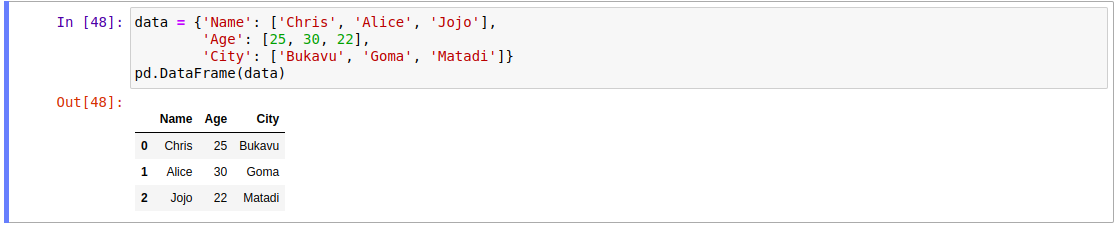
\includegraphics[width=16cm, height=3.7cm]{demoDataFrame}
\\

\textbf{Reading and Writing data.} Pandas offers versatile functionality which deal with various sources and formats. The common sources include : \newline
\textbf{- CSV files}: They are read and written like this : 
\begin{lstlisting}[style=stylepython]
 #Reading from CSV
 data = pd.read_csv('dafileName.csv') 
 #Writing to CSV
 data.to_csv('new_data_file_name.csv', index=False)
\end{lstlisting} 

\noindent \textbf{- Excel files} : 
 \begin{lstlisting}[style=stylepython]
# Reading from Excel
 data = pd.read_excel('dafileName.xlsx', sheet_name='Sheet1')

# Writing to Excel
 data.to_excel('new_data_file_name.xlsx', sheet_name='Sheet1', index=False)
 \end{lstlisting} 
 
 \textbf{- SQL Databases} :
  \begin{lstlisting}[style=stylepython]
# Reading from SQL database sqlite
connection = sqlite3.connect('my_database.db')
query = 'SELECT * FROM my_table'
data = pd.read_sql(query, connection)

# Writing to SQL database
data.to_sql('new_table', connection, if_exists='replace', index=False)
 \end{lstlisting}
 
In the same way, functions \textbf{read\_json, read\_html}  are also respectively used for dealing with the JSON and HTML data.\\

\textbf{- Data Cleaning.} Pandas uses several functions, among them we have drop\_duplicates(), fillna(). Which are used like this:
\begin{lstlisting}[style=stylepython]
# Removing duplicates
df = df.drop_duplicates()

# Handling missing values
df = df.fillna(0)
\end{lstlisting} 

\textbf{- Data Exploration}. Pandas provides methods for exploring the dataset, such as \textbf{head(), tail(), describe(), and info()}. Thus, the application will look like :
\begin{lstlisting}[style=stylepython]
data = {'A': [1, 2, 3, 4, 5],
'B': ['X', 'Y', 'Z', 'X', 'Y']}
df = pd.DataFrame(data)
# Display the summary statistics of numeric columns
print(df.describe()) 

              A
count  5.000000
mean   3.000000
std    1.581139
min    1.000000
25%    2.000000
50%    3.000000
75%    4.000000
max    5.000000
\end{lstlisting} 

\noindent \textbf{Data Manipulation}. Pandas performs the manipulation of tables as Excel using the pivot\_table() and merge() function perform combination operation for analysis.
Additionally it allows indexing, slicing, filtering, modifying data. Let's break into the demonstration:
\newline
\textbf{- Pivot table }:
\begin{lstlisting}[style=stylepython]
In [72] : df.pivot_table(index='B', values='A', aggfunc='mean')
print(pivot) 
     A
B     
X  2.5
Y  3.5
Z  3.0 

#The operation computed is the average measurement
\end{lstlisting} 

\textbf{- Merging} :
\begin{lstlisting}[style=stylepython]
 #Create two DataFrames
 data1 = {'Key': [1, 2, 3, 4, 5],
'Value1': ['A', 'B', 'C', 'D', 'E']}
data2 = {'Key': [3, 4, 5, 6, 7],
'Value2': ['X', 'Y', 'Z', 'U', 'V']}
df1 = pd.DataFrame(data1)
df2 = pd.DataFrame(data2)

# Perform combination-like operation
result = pd.merge(df1, df2, on='Key', how='left')
print(result) 

Key Value1 Value2
0    1      A    NaN
1    2      B    NaN
2    3      C      X
3    4      D      Y
4    5      E      Z
\end{lstlisting} 

\textbf{- Slicing}:
\begin{lstlisting}[style=stylepython] 
#Consider the example on the top about 
#name, age, city
# Slice specific rows and columns
  df.loc[1:3, 'Name':'Age']  
#From the second column till the threeth line 
#From the Name till the Age column
#The result gives this: 

Name  Age
1      Bob   30
2  Charlie   35
\end{lstlisting} 
Assume that we want to apply some characteristic on a column :
\begin{lstlisting}[style=stylepython]
# Create a new column based on an existing column
df['days'] = df['Age'].apply(lambda x: x * 360)
print(df)
# The result is like this: 
      Name   Age    City       days
0    Alice   25     New York   9000
1      Bob   30  Los Angeles  10800
2  Charlie   35      Chicago  12600
\end{lstlisting}

\textbf{- Modifying Data} : 
\begin{lstlisting}[style=stylepython]
df.loc[2, 'Name'] = "Jonathan"
print(df)
#The df becomes like this : 
Name  Age         City   days
0     Alice   25     New York   9000
1       Bob   30  Los Angeles  10800
2  Jonathan   35      Chicago  12600
\end{lstlisting} 

\subsubsection{Data Visualization With \textit{Matplotlib} and \textit{Seaborn}} 
\subsubsection*{\textit{Matplotlib}}
\textit{Matplotlib} is a open-source, flexible and customizable Python package used for creating 2D and 3D \footnote{mpl\_toolkits.mplots3d : \url{https://matplotlib.org/stable/tutorials/toolkits/mplot3d.html}, tools used for generating 3D plots } plotting having a high production-quality. In addition to this, it includes the capacity of saving images in different output formats (JPG, PNG, PS and others) \cite{tosi2009matplotlib}. 

To get started with it, we just go to the official page and download the dependencies \footnote{Matplotlib: \url{https://matplotlib.org/}}. However, for who are those using integrated development environment (\textit{IDE}) like \textit{Anaconda} \textit{numpy}, \textit{pandas}, and \textit{matplotlib} are incorporated inside.
When working with data visualization, the type of plot to choose should depend on the nature of the data. In the table \ref{tab:plotTypeDataTable} , the overview of types of plots and when to use them is given. However, some plots can be combined even though they are primarily made for whether categorical or numerical visualization. 

\noindent The usage of \textit{matplotlib} properties require a good manipulation of data, often done by the \textit{numpy} and \textit{pandas}. Let's break into examples of its usage: \newline
First all, the import of \textit{matplotlib} is required for any manipulation. It is done like this :
\begin{lstlisting}[style=stylepython]
import matplotlib.pyplot as plt #plt is also an alias
\end{lstlisting} 
 
\begin{lstlisting}[style=stylepython]
import matplotlib.pyplot as plt
import numpy as np

# Data
x = np.arange(1, 11)
y1 = x
y2 = x**2
y3 = np.sqrt(x)

# Create a figure with subplots (1row and 3 columns)
fig, axs = plt.subplots(1, 3, figsize=(15, 5))

# First Subplot: Line Plot   
axs[0].plot(x, y1, color='b', marker='o') # 'o' is a clue

#define legends
axs[0].set_title('Line Plot')
axs[0].set_xlabel('X-axis')
axs[0].set_ylabel('Y-axis')

# Second Subplot: Bar Plot
axs[1].bar(x, y2, color='g', alpha=0.6)
axs[1].set_title('Bar Plot')
axs[1].set_xlabel('X-axis')
axs[1].set_ylabel('Y-axis')

# Third Subplot: Scatter Plot 
axs[2].scatter(x, y3, color='r', marker='x')
axs[2].set_title('Scatter Plot')
axs[2].set_xlabel('X-axis')
axs[2].set_ylabel('Y-axis')

# Adjust subplot layout to prevent overlapping
plt.tight_layout()

# Display the figure
plt.show()
\end{lstlisting}  

\begin{figure}
	\centering
	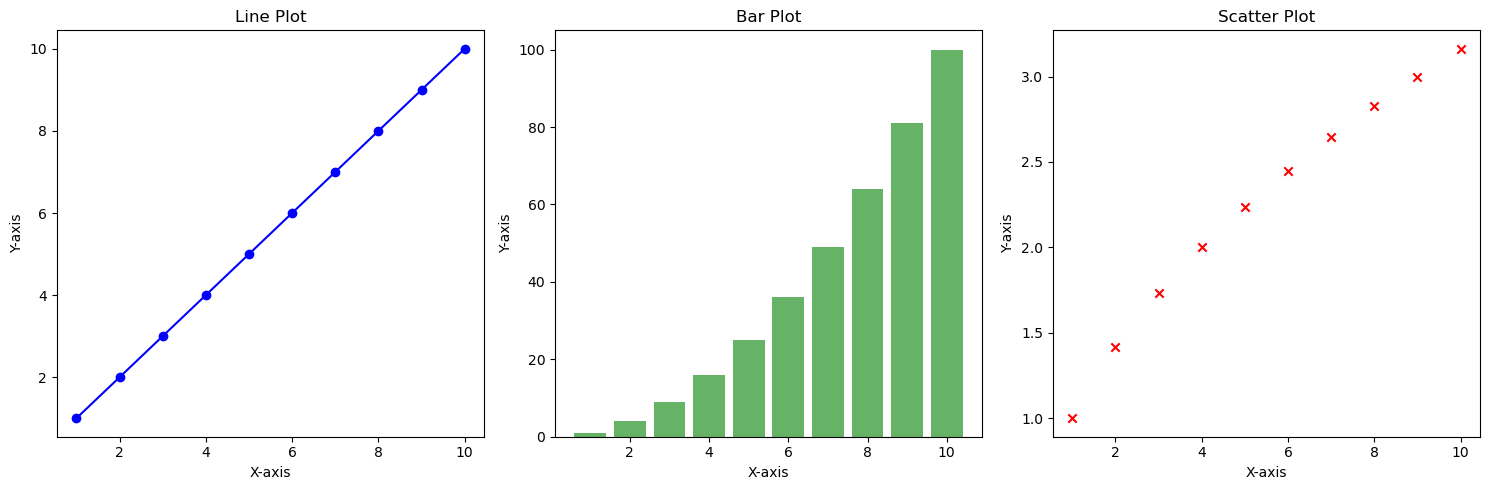
\includegraphics[width=1\linewidth]{matplotLibExample}
	\caption{How to use \textit{matplotlib} for visualization}
	\label{fig:matplotlibexample}
\end{figure} 

Additionally, \textit{matplotlib} is used for creating 3D as follows : 
\begin{lstlisting}[style=stylepython]
	from mpl_toolkits.mplot3d import Axes3D
	import matplotlib.pyplot as plt
	import numpy as np
	
	fig = plt.figure()
	ax = fig.add_subplot(111, projection='3d')
	
	x = np.random.rand(10)
	y = np.random.rand(10)
	z = np.random.rand(10)
	
	ax.scatter(x, y, z, c='r', marker='o')
	
	ax.set_xlabel('X-axis')
	ax.set_ylabel('Y-axis')
	ax.set_zlabel('Z-axis')
	
	plt.show()
\end{lstlisting} 
Notice that: \textit{matplotlib}, uses \textit{mpl\_toolkits} for integrating with 3D, since at its release it was creating 2D plots only. 
Besides, the difference observed in the code at axis where the function \textit{add\_subplot} receives 111 value as the first argument. It just defines that the plot will be a single for all 3 dimensions as shown in the figure \ref{fig:3ddimensionPlotlib}. 
\begin{figure}
	\centering
	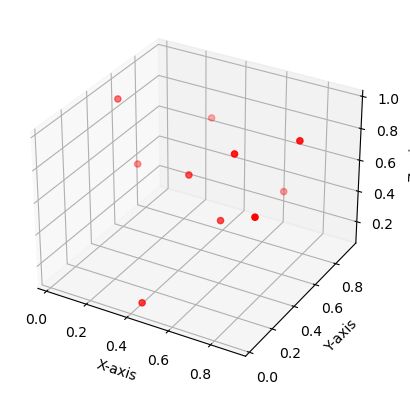
\includegraphics[width=0.7\linewidth]{3Ddimension}
	\caption{3D plot with Matplotlib}
	\label{fig:3ddimensionPlotlib}
\end{figure}

\begin{table}
	 % Color every other row
\begin{tabular}{|p{3cm}|p{3.5cm}|p{8cm}|} 
\hline
\hline 	
 Type of data	& Plot name & Utilities  \\

\hline
\hline
\centering
\multirow{10}{3cm}{{\large Categorical Data}} &   Bar Plot&  It is deal for showing the frequency or count of categorical data. \newline
Example: Comparing the number of apples, bananas, and oranges sold at a fruit stand \\ 
\cline{2-3} 

 & Pie Chart & Suitable for displaying parts of a whole. \newline
Example: Showing the composition of monthly expenses (eg. rent, groceries, utilities).\\ 
\cline{2-3}
 
& Stacked Bar Chart & Useful for comparing categories while also showing their composition\\
\hline
\centering
\multirow{14}{3cm}{\large Numerical Data} & Histogram & Visualizes the distribution of a single variable or continuous data.\newline 
Example : Analyzing the distribution of ages in a population\\
\cline{2-3}

& Box Plot & Displays the distribution and spread of numerical data\\
\cline{2-3}

 & Scatter Plot & Depicts relationships between two numerical variables \newline Example : Showing the correlation between the number of study hours and exam scores for multiple students.
 \\
\cline{2-3}

 & Line Plot & Shows changes in variable over a continuous range, often over time. \newline Example : Plotting stock prices over several months to visualize trends. \\
 \hline
\centering

\multirow{8}{3cm}{{\large Mixed Data}} & Violion Plot & Combines a box plot with a kernel density estimation to visualize the distribution. \newline Example: Comparing the distribution of test scores across different schools.\\
\cline{2-3}
& Heatmap & Useful for displaying relationship between multiple variables in matrix. \newline Example : Analyzing the correlation between various factors (eg., age, income, and education level) in a survey.\\
\hline 

\end{tabular}    
\caption{Choose the plot depending on data's nature}
\label{tab:plotTypeDataTable}
\end{table}

\subsubsection*{\textit{Seaborn}}
\textit{Seaborn} is another Python library for statistical data visualization, built on \textit{matplotlib}. It just provides properties able to create more informative an visually appealing graphics \cite{sial2021comparative}. To get started with it, we just visit the official page \footnote{Seaborn: \url{https://seaborn.pydata.org/}} which presents all steps required for installing. Alternatively, we can use an  the integrated development environment \textit{IDE} like \textit{Anaconda} once again, which already includes it. 

The following example shows how to combine both \textit{matplotlib} and \textit{seaborn}:  
\begin{lstlisting}[style=stylepython]
import matplotlib.pyplot as plt 
import seaborn as sns # Its how to start the 

# Create a Seaborn plot
sns.set(style="whitegrid")
tips = sns.load_dataset("tips")
ax = sns.barplot(x="day", y="total_bill", data=tips)

# Customize the plot using Matplotlib
ax.set(xlabel="Day of the Week", ylabel="Total Bill Amount")
plt.title("Average Total Bill Amount by Day")

#Save the plot as an image
plt.savefig("seaborn_customized_plot.png")
plt.show() # Show the plot
\end{lstlisting} 
The data used in the following code, named 'tips,' is provided for practice purposes. \textit{Seaborn} is used to generate the plot, while \textit{matplotlib} customizes it by adding a legend and saving the image generated in figure.


\subsubsection*{\large Machine learning with scikit-learn} 
  
Since Python programming language is establishing itself as one the most popular languages for scientific computing. Many and various libraries are developed inside making it more and more appealing \cite{pedregosa2011scikit}. \newline
\textit{Scikit-learn} is an open-source and commercially(usage - BSD license) machine learning library for the Python programming language. It was initially developed by David Counapeu in 2007 as part of the Google Summer of Code project. Since then, it has grown to become one the most popular and widely used Machine Learning libraries in Python ecosystem \cite{scikitlearnCode1}.   
The techniques and properties used inside of it, allows it to predictive data analysis by performing the  classification, regression, clustering, preprocessing and more other tasks.\newline
To get started with it as usually, the official page present all the steps for downloading all the packages or using \textit{IDE} like \textit{Anaconda} which encompasses it. 

Before using its functions we have to initialize the by import the class which includes the methods and properties achieving a given task. For example, suppose that we are about to process data a class called \textit{StandardScaler} can be useful \textbf{when the dataset contains features with different scales} . Then, it standardizes the data, making it have a mean of 0 and standard deviation of 1, assuring that all features have the same scale.
\begin{lstlisting}[style=stylepython]
In[2]:  from sklearn.preprocessing import StandardScaler
	import numpy as np
	
	# Example data
	data = np.array([[1.0, 2.0, 3.0],
	[4.0, 5.0, 6.0],
	[7.0, 8.0, 9.0]])
	
	# Create a StandardScaler instance
	scaler = StandardScaler()
	
	# Fit the scaler to the data and transform the data
	data_standardized = scaler.fit_transform(data)
	
	print("Original Data:")
	print(data)
	print("Standardized Data:")
	print(data_standardized)  
	
Out[2]:
	
	Original Data:
	[[1. 2. 3.]
	[4. 5. 6.]
	[7. 8. 9.]]
	Standardized Data:
	[[-1.22474487 -1.22474487 -1.22474487]
	[ 0.          0.          0.        ]
	[ 1.22474487  1.22474487  1.22474487]]
	
\end{lstlisting}
  We just notice that, this time, all the standardized data have a mean close to 0 and a standard deviation close to 1. For that, the data become centered around zero and have now consistent units of measurement. \newline
  Additionally, the \textit{\textbf{fitstransform()}} method on the object, defines both fitting and transformation process. Actually, the \textit{\textbf{fit()}} method computes the mean and standard deviation of the trained data and \textit{\textbf{transform()}} method scales the trained data based on the mean and standard deviation. Indeed,  \textit{fitstransform()} includes all both. \newline Actually, the explanations about training, fitting and others principles concerning a model are going to be tackled in the section 3 untitled :'Thinking in machine learning'.
  
\subsection{Summary concerning the tools and frameworks}
The completion of this project necessitated the utilization of various dependencies, tools, frameworks. These resources were instrumental in realizing the project's objectives. Notably, they were categorized into two main areas: those integral to the core functionality and others relevant to the user side, distinguishing the back-end from the front-end. Moreover, the project involved tools for data analysis and predictive modeling. The structure of these tools is presented in the  table \ref{tableStructuring}  for more clarity.
  \\
\begin{table}
\begin{tabular}{|p{4.1cm}|p{4cm}|p{6cm}|}
	\cline{2-3} 
    \multicolumn{1}{c|}{} & \textbf{Tools}   & \textbf{Roles}  \\
	\hline
\multirow{11}{4cm}{\textbf{Data analysis and Machine Learning libraries}}	& \textit{Numpy} & Scientific computing library   \\ 
	\cline{2-3} 
	& \textit{Panda}  & Data manipulation and
	analysis library  \\ 
	\cline{2-3} 
	& \textit{Matplotlib}  & Python library used for 2D and 3D data visualization   \\ 
	\cline{2-3}  
	& \textit{Seaborn} & Another Python library for statistical data visualization, built on \textit{matplotlib}.\\
	\cline{2-3} 
		& \textit{Scickit-learn}  & Machine learning machine learning library \\
	\hline
	\multirow{5}{4cm}{\textbf{Programming Languages (\textit{Front-end} and \textit{Back-end})}}& \textit{Django} Python & Python framework for developing web applications and \textit{APIs}\\ 
	 \cline{2-3}
	 & HTML & Maker of web pages by providing
	 its structure and content \\ 
	 \cline{2-3}
	 & CS & Styling the content\\ 
	 \cline{2-3}
	 & JS & Rendering web pages interactive and dynamic \\
	 \hline
	
\end{tabular}
\caption{Structuring the tools} 
\label{tableStructuring}
\end{table} 
\section{Description of the methodology and approach}
Choosing a right methodology including approaches and methods to use, is an important task. However, the nature of environment defers and leads to challenging evaluation before determining the fit one. Thus, since this project investigates in Machine Learning project, the appealing methodology chosen for its achievement is inspired from MLOps(ML Operating systems).\\

\subsection{\textbf{{\large  ML operating systems}}} 
ML endeavors aim to deal with their projects from development till the production step. However, a large number of projects based on ML don't reach the final step according to their expectations. Actually, the paradigm of MLOps came to face this issue \cite{kreuzberger2023machine}. For that, it is a set of principles, best practices and concepts, and development culture that provide an end-to-end machine learning development process to design, build and manage reproducible, testable and evolvable ML-powered software. 

Furthermore, MLops involves the union of many disciples, including Machine learning, software engineering (concerning DevOps too), data engineering as clarified in figure \ref{fig:mlopsdisciplines}.
\begin{figure}[h!]
	\centering
	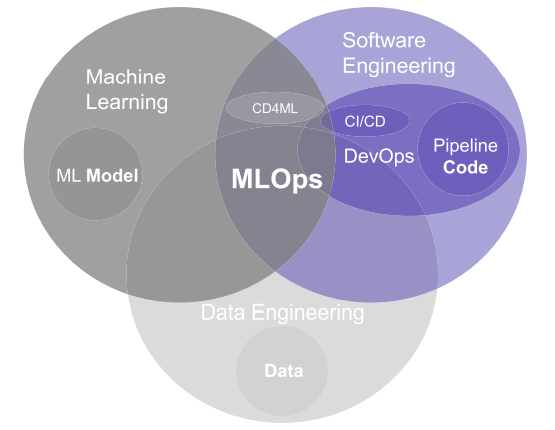
\includegraphics[width=1\linewidth]{../../../Books/Report/MLopsDisciplines}
	\caption{Intersection of disciplines in MLops}
	\label{fig:mlopsdisciplines}
\end{figure} 

\textbf The {Machine learning part} is dealt by \textbf{data scientists} and have the principle role of building the models that address the business question or needs. While \textbf{Data Engineering} is conducted by data engineers making sure that data pipelines which are the core of the ML model life cycle, are in turn and clean. Next, the \textbf{Software engineering}, encompasses \textbf{software engineers} not highly concerned by the machine learning model building since they bring ML problem into a well-engineered product (into applications). 
In the other hand, \textbf{DevOps} is directed by DevOps engineers who bridges the gap between development and operations, granting that updates are continuously integrated and the development is still pursued (referring to \textit{CI/CS}, Continuous Integration et Development ). \\

All these disciplines work together to follow the ML life cycle, demonstrating that ML endeavors are on ongoing process within the same project for ensuring that it is more impacting in terms of results. As shown in the figure \ref{fig:mllifecyle} the ML life cycle follows several steps resumed in the following points :
\begin{itemize}  
	\item Definition of the object and specification 
	\item Data Collection 
	\item Preparation and exploratory Data Analysis
	\item Model Training \& Evaluation
	\item Model Deployment 
	\item Model Monitoring 
\end{itemize} 
\begin{figure}[h!]
	\centering
	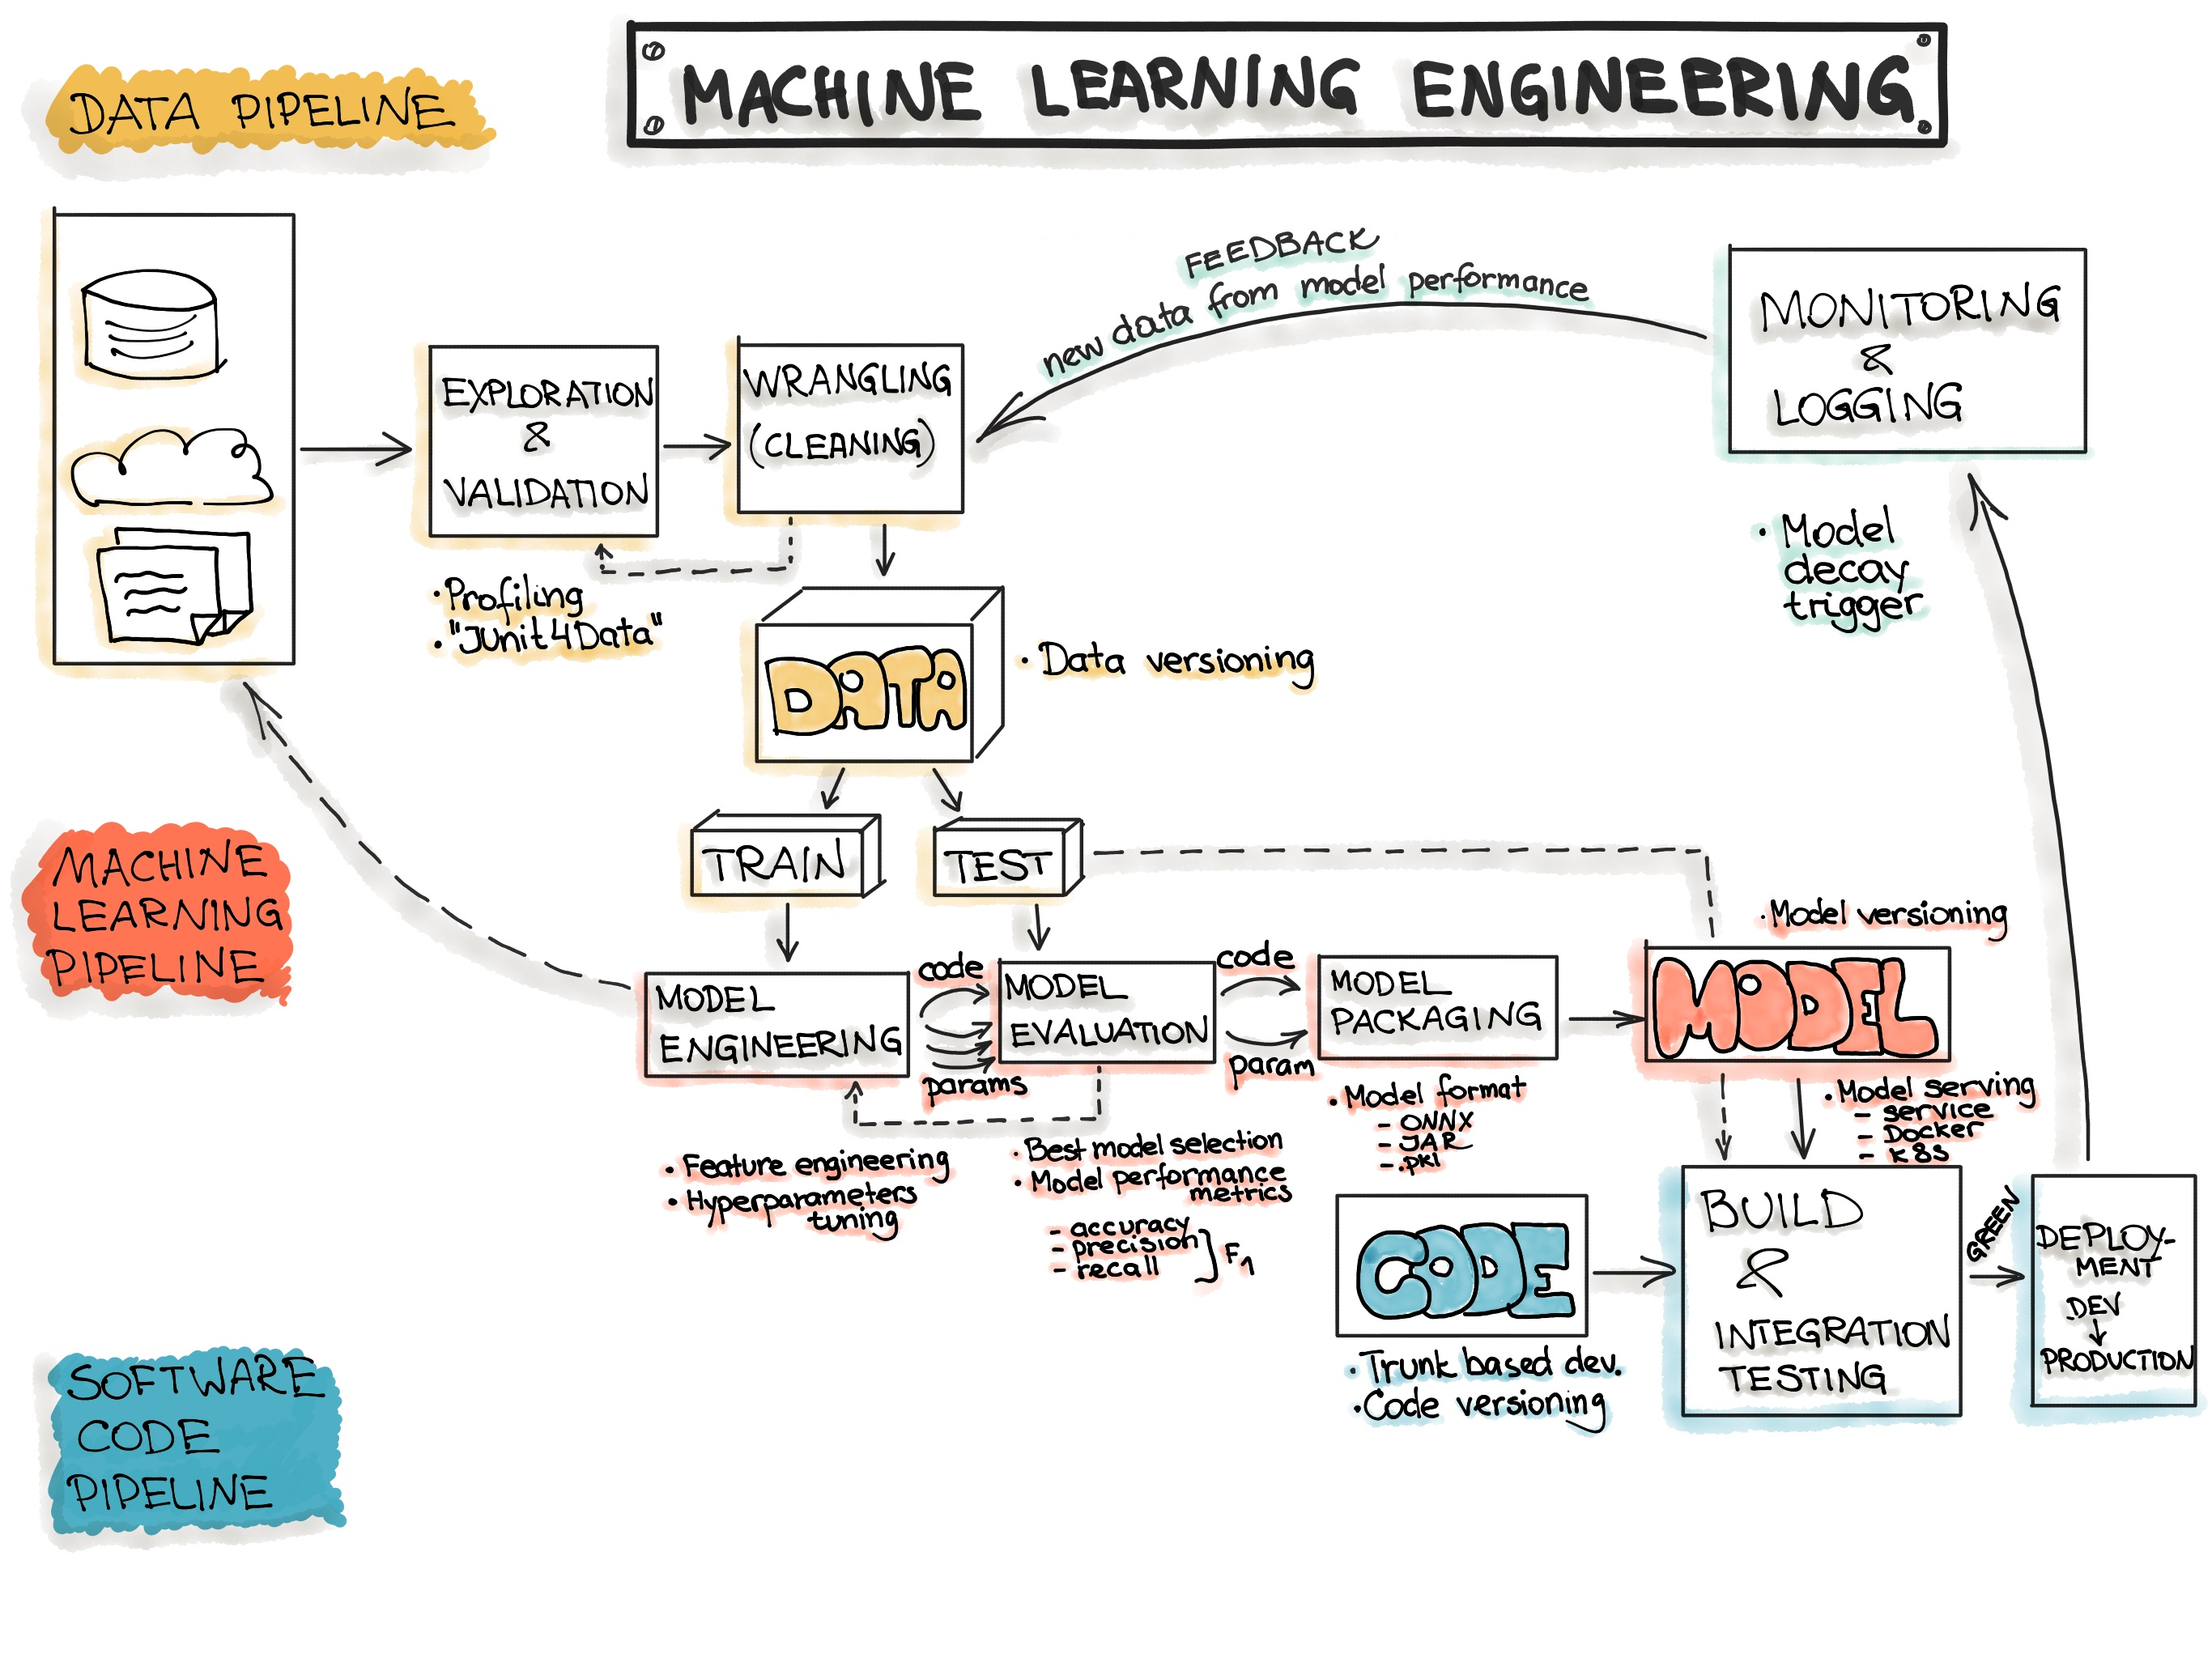
\includegraphics[width=1\linewidth]{ml-engineeringInspiration}
	\caption{Machine Learning Workflow}
	\label{fig:mllifecyle}
\end{figure}
\subsection{Definition of the object and specification}
The definition of the object and specification is start stage where details about the problem is given in the clear way for facilitating the ML development. This task is associated to Business stakeholders who define the goal pursued. 

\subsection{Gathering data}
At this step, raw data are collected from various data pipeline(sources) depending on interests of project and environment. Thus, data's source can be :  
(a) Databases, including data structured in relational databases like SQL and NoSQL databases. Actually, databases is mostly preferable source since they give structured data well-suited for analysis;

(b)  Files (CSV, Text Files). This mean is highly used. It requires important analysis of the content for being aware of how and what part to extract (as spreadsheets for Excel), separated values (as for CSV files).

(c) APis. They are also the common use for structured data( in JSON, XML format) , leveraging web services for providing data to third parties or internal parties of the system \cite{dataScienceMLeric}.

(d) Web Scrapping. This mean refers to techniques used for collecting data from web sites (sometimes illegally) and structure it into spreadsheets, CSV or others simple means \cite{sirisuriya2015comparative}. It's more appreciated when data are not available from the APIs. That being, some applications performs like 

(e) Images and videos : Images, videos are generated from cameras, satellites and other imaging devices. Thus, they are useful in specific tasks of ML like classification of taxonomy videos \cite{reviewVideo2020}. 
Many others means exist like surveys and questionnaires, audio data, however the guidance is problem to address. 
\\
Once the data are collected, it stored in \textbf{dataset} where they are subjected to manipulation and analysis.
\subsection{Data preparation and wrangling}
The preparation refers to two main tasks : The data pre-processing(wrangling) and data exploration . The data pre-prepocessing involves the learning of nature of the data, its characteristics, types format and quality, that consequently lead to better outcome. While, The data wrangling consist of cleaning necessary data. 

On the other hand,\textbf{the exploratory data analysis} process aims to receive collected and cleaned data and facilitates the visualization that can be helpful in detection of outliers, identification of clusters and trends \cite{unwin2020data}.
\subsection{Model building and selection}

\newpage
 %\bibliographystyle{apacite} % or whatever citation style you choose
\bibliographystyle{plain}
\bibliography{bibliofile.bib}
	
\newpage	
	
	
	
	
	
	
	
\end{document}